%%%%%%%%%%%%%%%%%%%%%%%%%%%%%%%%%%%%%%%%%%%%%%%%%%%%%%%%%%%%%%%%%%%%%%%%%%%%%%%%
%%%%%%%%%%%%%%%%%%%%%%%%%%%%%%%%%%%%%%%%%%%%%%%%%%%%%%%%%%%%%%%%%%%%%%%%%%%%%%%%
%%%%%%%%%%%%%%%%%%%%%%%%%%%%%%%%%%%%%%%%%%%%%%%%%%%%%%%%%%%%%%%%%%%%%%%%%%%%%%%%

\documentclass[
	11pt, % Set the default font size, options include: 8pt, 9pt, 10pt, 11pt, 12pt, 14pt, 17pt, 20pt
	%t, % Uncomment to vertically align all slide content to the top of the slide, rather than the default centered
	%aspectratio=169, % Uncomment to set the aspect ratio to a 16:9 ratio which matches the aspect ratio of 1080p and 4K screens and projectors
]{beamer}

% Theme %%%%%%%%%%%%%%%%%%%%%%%%%%%%%%%%%%%%%%%%%%%%%%%%%%%%%%%%%%%%%%%%%%%%%%%%
\usetheme{default}
% Color theme %%%%%%%%%%%%%%%%%%%%%%%%%%%%%%%%%%%%%%%%%%%%%%%%%%%%%%%%%%%%%%%%%%
\usecolortheme{whale}
% Font theme %%%%%%%%%%%%%%%%%%%%%%%%%%%%%%%%%%%%%%%%%%%%%%%%%%%%%%%%%%%%%%%%%%%
\usefonttheme{default}

% Packages %%%%%%%%%%%%%%%%%%%%%%%%%%%%%%%%%%%%%%%%%%%%%%%%%%%%%%%%%%%%%%%%%%%%%
%%%%%%%%%%%%%%%%%%%%%%%%%%%%%%%%%%%%%%%%%%%%%%%%%%%%%%%%%%%%%%%%%%%%%%%%%%%%%%%%
\usepackage{booktabs} 
\usepackage{bookmark}
\usepackage{hyperref}
\usepackage{xcolor}
\usepackage{xurl}

% Presentation metadata %%%%%%%%%%%%%%%%%%%%%%%%%%%%%%%%%%%%%%%%%%%%%%%%%%%%%%%%
%%%%%%%%%%%%%%%%%%%%%%%%%%%%%%%%%%%%%%%%%%%%%%%%%%%%%%%%%%%%%%%%%%%%%%%%%%%%%%%%
\title{Data Anonymization for Open Science}
\subtitle{useR! 2024}
\author{Jiří~Novák\inst{1,2} \and Marko~Miletić\inst{3} \newline
\and Oscar~Thees\inst{2} \and Alžběta~Beranová\inst{4}}
\date{July 8, 2024}
\institute{\inst{1} University of Zurich \inst{2} University of Applied
Sciences Northwestern Switzerland \and \inst{3} Bern University of
Applied Sciences \inst{4} Czech Statistical Office}

\titlegraphic{
   
\includegraphics[width=2cm]{style/UZH.jpg}
   \hspace*{2cm}~%
   
\includegraphics[width=2cm]{style/FHNW.png}
   \hspace*{2cm}~%
   
\includegraphics[width=1cm]{style/BFH.png}
   }

% Start of the presentation %%%%%%%%%%%%%%%%%%%%%%%%%%%%%%%%%%%%%%%%%%%%%%%%%%%%
%%%%%%%%%%%%%%%%%%%%%%%%%%%%%%%%%%%%%%%%%%%%%%%%%%%%%%%%%%%%%%%%%%%%%%%%%%%%%%%%
%%%%%%%%%%%%%%%%%%%%%%%%%%%%%%%%%%%%%%%%%%%%%%%%%%%%%%%%%%%%%%%%%%%%%%%%%%%%%%%%
\begin{document}

% Title %%%%%%%%%%%%%%%%%%%%%%%%%%%%%%%%%%%%%%%%%%%%%%%%%%%%%%%%%%%%%%%%%%%%%%%%
\begin{frame}
	\titlepage % Output the title slide, automatically created using the text entered in the PRESENTATION INFORMATION block above
\end{frame}

% License %%%%%%%%%%%%%%%%%%%%%%%%%%%%%%%%%%%%%%%%%%%%%%%%%%%%%%%%%%%%%%%%%%%%%%
\begin{frame}
\vspace{12em}

Jiří Novák CC BY-NC-ND (2024)


\includegraphics{style/by-nc-nd.png}

This license enables reusers to copy and distribute the material in any
medium or format in unadapted form only, for noncommercial purposes
only, and only so long as attribution is given to the creator.
\end{frame}

% Table of Content %%%%%%%%%%%%%%%%%%%%%%%%%%%%%%%%%%%%%%%%%%%%%%%%%%%%%%%%%%%%%
\begin{frame}{Table of Content}
\Large
\begin{enumerate}
  \item General methodological overview
  \item Disclosure control methods
  \begin{enumerate}[A.]
    \large
    \item Non-perturbation methods
    \item Perturbation methods
    \item Synthetic methods
    \begin{itemize}
    \large
      \item Generating synthetic data using synthpop
      \item Generating synthetic data using simPop
      \item Generating synthetic data with GANs
    \end{itemize}
  \end{enumerate}
\end{enumerate}
\end{frame}

% Data Anonymization in which context? %%%%%%%%%%%%%%%%%%%%%%%%%%%%%%%%%%%%%%%%%
\begin{frame}{Data Anonymization in which context?}
\phantomsection\label{data-anonymization-in-which-context}
This tutorial is about Data Anonymization in the context of the field of
\textbf{Statistical Disclosure Control} (SDC).

SDC is also known as Statistical disclosure limitation or Disclosure
avoidance.

\vspace{1cm}

\textbf{Statistical Disclosure Control} seeks to protect statistical
data in such a way that they can be released without giving away
confidential information that can be linked to specific individuals or
entities.
\end{frame}

% Importance of Data Anonymization %%%%%%%%%%%%%%%%%%%%%%%%%%%%%%%%%%%%%%%%%%%%%
\begin{frame}{Importance of Data Anonymization}
\phantomsection\label{importance-of-data-anonymization}
There are several main reasons:

\begin{enumerate}
\item
  \textbf{Principle} It is a fundamental principle of Official
  Statistics that the statistical records of individual persons,
  businesses, or events used to produce Official Statistics are strictly
  confidential and to be used only for statistical purposes.
\item
  \textbf{Legal} Legislation imposes a legal obligation to protect
  individual business and personal data. Legal frameworks regulate what
  is allowed and what is not allowed regarding the publication of
  private information.
\item
  \textbf{Quality} Respondents need confidence in the preservation of
  the confidentiality of individual information. If they do not trust
  the confidentiality of the data, they may not provide accurate
  information.
\item
  \textbf{Ethical} Disclosing information that can be linked to specific
  individuals or entities is unethical.
\end{enumerate}
\end{frame}

% Relevance to Open Science %%%%%%%%%%%%%%%%%%%%%%%%%%%%%%%%%%%%%%%%%%%%%%%%%%%%
\begin{frame}{Relevance to Open Science}
\phantomsection\label{relevance-to-open-science}
\textbf{Open Science}, \textbf{Open Access}, \textbf{Open Data} are
important trends in the scientific community.

Research data that results from publicly funded research should be
\textbf{FAIR}: \newline \textbf{findable}, \textbf{accessible},
\textbf{interoperable}, \textbf{reusable}

\begin{itemize}
\item
  therefore replicable, transparent, trustworthy
\item
  Principle: \textbf{As open as possible, as closed as necessary}
\item
  Enables data sharing and collaboration
\item
  Facilitates reproducible research
\item
  Balances transparency with privacy
\end{itemize}

\href{https://eur-lex.europa.eu/eli/reco/2018/790/oj}{\color{blue}\underline{Commission Recommendation (EU) 2018/790 on access to and preservation}}
\href{https://eur-lex.europa.eu/eli/reco/2018/790/oj}{\color{blue}\underline{of scientific information}}
\end{frame}

% Outputs to protect %%%%%%%%%%%%%%%%%%%%%%%%%%%%%%%%%%%%%%%%%%%%%%%%%%%%%%%%%%%
\begin{frame}{Outputs to protect}
\phantomsection\label{outputs-to-protect}
Different outputs require different approaches to SDC and different
mixtures of tools.

\begin{itemize}
\tightlist
\item
  \textbf{Macrodata} (Tabular data)
\item
  \textbf{Microdata}
\item
  \textbf{Dynamic databases}
\item
  \textbf{Statistical analyses}
\end{itemize}

\vspace{1cm}

\textbf{Disclaimer}: Imposing a single solution for all types of data is
not possible. \newline This tutorial will focus on Microdata and Tabular
data.
\end{frame}

% Key Concepts %%%%%%%%%%%%%%%%%%%%%%%%%%%%%%%%%%%%%%%%%%%%%%%%%%%%%%%%%%%%%%%%%
\begin{frame}{Key Concepts}
\phantomsection\label{key-concepts}
Key Concepts are:

\begin{itemize}
\tightlist
\item
  \textbf{Disclosure}

  \begin{itemize}
  \tightlist
  \item
    A disclosure occurs when a person or an organisation recognises or
    learns somethingthat they did not know already about another person
    or organisation, via released data.
  \end{itemize}
\end{itemize}

\pause

\begin{itemize}
\tightlist
\item
  \textbf{Re-identification risk}

  \begin{itemize}
  \tightlist
  \item
    Re-identification risk is the risk that an intruder can link a
    record in the released data to a specific individual in the
    population.
  \end{itemize}
\end{itemize}

\pause

\begin{itemize}
\tightlist
\item
  \textbf{Data utility}

  \begin{itemize}
  \tightlist
  \item
    Data utility is the usefulness of the data for the intended purpose.
  \end{itemize}
\end{itemize}
\end{frame}

% Disclosure %%%%%%%%%%%%%%%%%%%%%%%%%%%%%%%%%%%%%%%%%%%%%%%%%%%%%%%%%%%%%%%%%%%
\begin{frame}{Disclosure}
\phantomsection\label{disclosure}
A disclosure occurs when a person or an organisation recognises or
learns something that they did not know already about another person or
organisation, via released data.

Types of disclosure risk:

\begin{enumerate}
[(1)]
\tightlist
\item
  \textbf{Identity disclosure} Revealing the identity of an individual.
  \vspace{0.5cm}
\item
  \textbf{Attribute disclosure} Revealing sensitive attributes of an
  individual. \vspace{0.5cm}
\item
  \textbf{Inferential disclosure} Making inferences about an individual
  based on the released data.
\end{enumerate}
\end{frame}

% Disclosure %%%%%%%%%%%%%%%%%%%%%%%%%%%%%%%%%%%%%%%%%%%%%%%%%%%%%%%%%%%%%%%%%%%
\begin{frame}{Disclosure}
\phantomsection\label{disclosure-1}
Types of disclosure risk:

\begin{enumerate}
[(1)]
\tightlist
\item
  \textbf{Identity disclosure}
\end{enumerate}

\vspace{-2em}
\begin{table}[ht] 
\centering
\begin{tabular}[t]{lccc}
\toprule
Residency&Age&Sex&Occupation\\
\midrule
Salzburg&50&Male&Professor\\
\bottomrule
\end{tabular}
\end{table}

\begin{enumerate}
[(1)]
\setcounter{enumi}{1}
\tightlist
\item
  \textbf{Attribute disclosure}
\end{enumerate}

\vspace{-2em}
\begin{table}[ht]
\centering
\begin{tabular}[t]{lccc}
\toprule
Group&Males&Females&Total\\
\midrule
Football fans&22&0&22\\
Non Football fan&93&85&178\\
Total&115&85&200\\
\bottomrule
\end{tabular}
\end{table}
\end{frame}

% Risk and utility %%%%%%%%%%%%%%%%%%%%%%%%%%%%%%%%%%%%%%%%%%%%%%%%%%%%%%%%%%%%%
\begin{frame}{Risk and utility}
\phantomsection\label{risk-and-utility}
SDC seeks to optimise the trade-off between the disclosure risk and the
utility of the protected released data.

\begin{itemize}
\item
  \textbf{Risk}: the probability of a disclosure event occurring.
\item
  \textbf{Utility}: the usefulness of the data for the intended purpose.
\end{itemize}

The goal is to find a balance between risk and utility.
\end{frame}

% Risk-utility trade-off %%%%%%%%%%%%%%%%%%%%%%%%%%%%%%%%%%%%%%%%%%%%%%%%%%%%%%%
\begin{frame}{Risk-utility trade-off}
\phantomsection\label{risk-utility-trade-off}
\begin{figure}[H]

{\centering 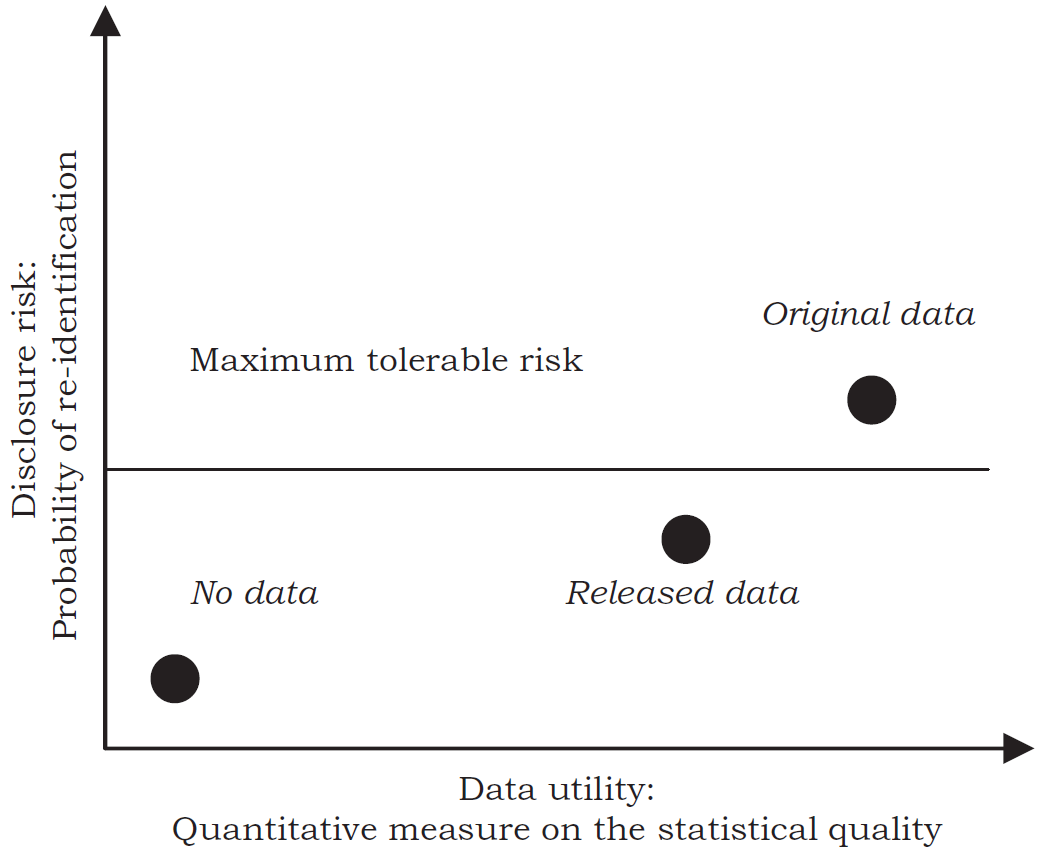
\includegraphics[width=0.5\textwidth,height=\textheight]{gallery/R-U confidentiality map.png}}

\caption{R-U confidentiality map (Duncan et al.,2001)}

\end{figure}%
\end{frame}

% Disclosure risk %%%%%%%%%%%%%%%%%%%%%%%%%%%%%%%%%%%%%%%%%%%%%%%%%%%%%%%%%%%%%%
\begin{frame}{Disclosure risk}
\phantomsection\label{disclosure-risk}
A unit is at risk of disclosure when it cannot be confused with several
other units in the data set.

\begin{itemize}
\item
  \textbf{k-anonymity} A data set is said to satisfy k-anonymity for k
  \textgreater{} 1 if, for each combination of values of
  quasi-identifiers (e.g.~name, address, age, gender, etc.), at least k
  records exist in the data set sharing that combination.
\item
  Ensures that each record is indistinguishable from at least k-1 other
  records with respect to the quasi-identifiers.
\end{itemize}

More robust approaches:

\begin{itemize}
\item
  \textbf{l-Diversity} Extends k-anonymity by ensuring that the
  sensitive attribute has at least l well-represented values
\item
  \textbf{t-Closeness} Ensures that the distribution of the sensitive
  attribute in any equivalence class is close to the distribution in the
  entire dataset
\end{itemize}
\end{frame}

% Attacker Scenarios %%%%%%%%%%%%%%%%%%%%%%%%%%%%%%%%%%%%%%%%%%%%%%%%%%%%%%%%%%%
\begin{frame}{Attacker Scenarios}
\phantomsection\label{attacker-scenarios}
\textbf{Data Intruder}: An attacker who tries to re-identify individuals
using the anonymized dataset and auxiliary information. For example,
consider a dataset of anonymized medical records. An intruder might use
publicly available information, like voter registration lists, to link
unique combinations of quasi-identifiers (such as age, gender, and zip
code) to re-identify individuals.

\textbf{Data Linkage}: This scenario involves an attacker who combines
multiple datasets to enhance the chances of re-identification. For
example, if an attacker has access to an anonymized dataset from a
hospital and another dataset from a social media platform, they might
link these datasets through common quasi-identifiers to re-identify
patients.

\textbf{Background Knowledge}: An attacker might use their own knowledge
about certain individuals to identify them in a dataset. For example, if
someone knows a particular person's age, job title, and city, they might
find a matching record in an anonymized employment dataset, thereby
re-identifying that individual.
\end{frame}

% Variables %%%%%%%%%%%%%%%%%%%%%%%%%%%%%%%%%%%%%%%%%%%%%%%%%%%%%%%%%%%%%%%%%%%%
\begin{frame}{Variables}
\phantomsection\label{variables}
\begin{enumerate}
\item
  \textbf{Identifiers} - variables that can directly identify an
  individual
\item
  \textbf{Quasi-identifiers} or \textbf{key variables} - these variables
  don't identify individuals on their own but can do so when combined
  with other quasi-identifiers
\item
  \textbf{Confidential outcome variables} - variables that contain
  sensitive information that should be protected
\item
  \textbf{Non-confidential outcome variables} - these are variables that
  are not sensitive and don't risk the privacy of individuals if
  disclosed
\end{enumerate}
\end{frame}

% Disclosure control methods %%%%%%%%%%%%%%%%%%%%%%%%%%%%%%%%%%%%%%%%%%%%%%%%%%%
\begin{frame}{Disclosure control methods}
\phantomsection\label{disclosure-control-methods}
\begin{enumerate}
\tightlist
\item
  \textbf{Masking original data}

  \begin{enumerate}
  [i.]
  \tightlist
  \item
    \textbf{Non-perturbative masking} - Methods that alter data to hide
    identities without changing its actual values
  \item
    \textbf{Perturbative masking} - Methods that add noise or alter data
    values to prevent identification
  \end{enumerate}
\item
  \textbf{Generating synthetic data}

  \begin{enumerate}
  [i.]
  \tightlist
  \item
    \textbf{Parametric methods} - Techniques that use statistical models
    based on the data's distribution to generate synthetic data.
  \item
    \textbf{Non-parametric methods} Techniques that do not assume an
    underlying distribution, using methods like bootstrapping to
    generate synthetic data.
  \item
    \textbf{Generative Adversarial Networks (GANs)} Advanced machine
    learning models that generate highly realistic synthetic data by
    training two neural networks in tandem.
  \end{enumerate}
\end{enumerate}
\end{frame}

% Packages for SDC - Microdata (Unit-level data) %%%%%%%%%%%%%%%%%%%%%%%%%%%%%%%
\begin{frame}{Packages for SDC - Microdata (Unit-level data)}
\phantomsection\label{packages-for-sdc---microdata-unit-level-data}
\href{https://cran.r-project.org/web/packages/sdcMicro/index.html}{\color{blue}\underline{\textbf{sdcMicro}}}
can be used to anonymize data, i.e.~to create anonymized files for
public and scientific use. It implements a wide range of methods for
anonymizing categorical and continuous (key) variables. The package also
contains a graphical user interface, which is available by calling the
function sdcGUI.

\href{https://cran.r-project.org/web/packages/simPop/index.html}{\color{blue}\underline{\textbf{simPop}}}
using linear and robust regression methods, random forests (and many
more methods) to simulate synthetic data from given complex data. It is
also suitable to produce synthetic data when the data have hierarchical
and cluster information (such as persons in households) as well as when
the data had been collected with a complex sampling design. It makes use
of parallel computing internally.

\href{https://cran.r-project.org/web/packages/synthpop/index.html}{\color{blue}\underline{\textbf{synthpop}}}
using regression tree methods to simulate synthetic data from given
data. It~is suitable to produce synthetic data when the data have no
hierarchical and cluster information (such as households) as well as
when the data does not collected with a~complex sampling design.
\end{frame}

% Packages for SDC - Tabular data (Aggregated data) %%%%%%%%%%%%%%%%%%%%%%%%%%%%
\begin{frame}{Packages for SDC - Tabular data (Aggregated data)}
\phantomsection\label{packages-for-sdc---tabular-data-aggregated-data}
\href{https://cran.r-project.org/web/packages/sdcTable/index.html}{\color{blue}\underline{\textbf{sdcTable}}}
can be used to provide confidential (hierarchical) tabular data. It
includes the HITAS and the HYPERCUBE technique and uses linear
programming packages (Rglpk and lpSolveAPI) for solving (a large amount
of) linear programs.

\href{https://cran.r-project.org/web/packages/sdcSpatial/index.html}{\color{blue}\underline{\textbf{sdcSpatial}}}
can be used to smooth or/and suppress raster cells in a map. This is
useful when plotting raster-based counts on a map. sdcHierarchies
provides methods to generate, modify, import and convert nested
hierarchies that are often used when defining inputs for statistical
disclosure control methods.

\href{https://cran.r-project.org/web/packages/SmallCountRounding/index.html}{\color{blue}\underline{\textbf{SmallCountRounding}}}
can be used to protect frequency tables by rounding necessary inner
cells so that cross-classifications to be published are safe.

\href{https://cran.r-project.org/web/packages/GaussSuppression/index.html}{\color{blue}\underline{\textbf{GaussSuppression}}}
can be used to protect tables by suppression using the Gaussian
elimination secondary suppression algorithm.
\end{frame}

% Non-perturbation methods %%%%%%%%%%%%%%%%%%%%%%%%%%%%%%%%%%%%%%%%%%%%%%%%%%%%%
\begin{frame}{Non-perturbation methods}
\phantomsection\label{non-perturbation-methods}
Non-perturbative masking does not rely on distortion of the original
data but on partial suppressions or reductions of detail.

\begin{table}[ht]   
\centering  
\begin{tabular}[t]{lccc}    
\toprule    
 Method & Continuous data & Categorical data&\\ 
\midrule    
 Sampling  & & X &\\    
 Global recoding & X & X &\\    
 Top and bottom coding& X & X &\\   
 Local suppression & & X &\\    
\bottomrule 
\end{tabular}   
\caption{Non-perturbative methods vs. data types}   
\end{table}
\end{frame}

% sdcMicro %%%%%%%%%%%%%%%%%%%%%%%%%%%%%%%%%%%%%%%%%%%%%%%%%%%%%%%%%%%%%%%%%%%%%
\begin{frame}{sdcMicro}
\phantomsection\label{sdcmicro}
\begin{itemize}
\item
  sdcMicro is an R package for statistical disclosure control.
\item
  \url{https://cran.r-project.org/web/packages/sdcMicro/index.html}
\item
  \url{https://github.com/sdcTools/sdcMicro}
\end{itemize}
\end{frame}

% sdcMicro %%%%%%%%%%%%%%%%%%%%%%%%%%%%%%%%%%%%%%%%%%%%%%%%%%%%%%%%%%%%%%%%%%%%%
\begin{frame}{sdcMicro}
\phantomsection\label{sdcmicro-1}

\begin{figure}[H]
{\centering 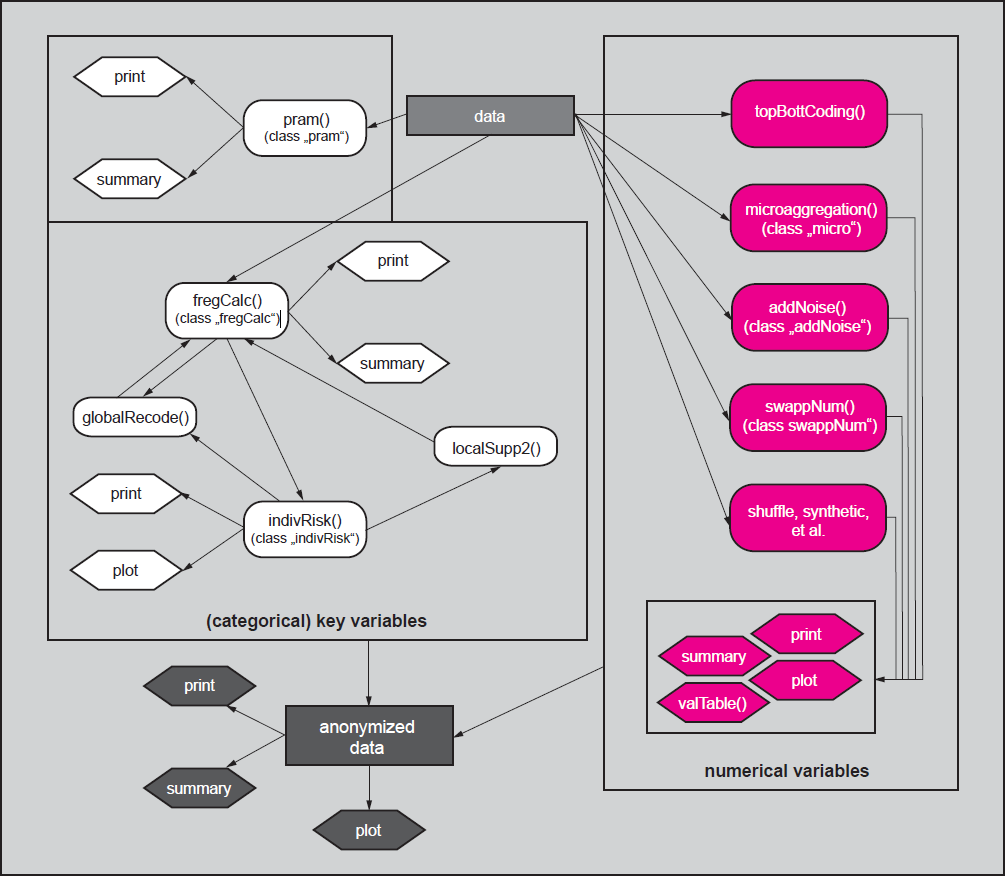
\includegraphics[width=0.55\textwidth,height=\textheight]{gallery/sdcMicro.png}
}
\caption{Certain procedures in package \emph{sdcMicro} and their
relationship}
\end{figure}%

\end{frame}

% Perturbation methods %%%%%%%%%%%%%%%%%%%%%%%%%%%%%%%%%%%%%%%%%%%%%%%%%%%%%%%%%
\begin{frame}{Perturbation methods}
\phantomsection\label{perturbation-methods}
\begin{itemize}
\item
  \color{red}{sdcMicro}
\end{itemize}
\end{frame}

% Synthetic methods %%%%%%%%%%%%%%%%%%%%%%%%%%%%%%%%%%%%%%%%%%%%%%%%%%%%%%%%%%%%
\begin{frame}{Synthetic methods}
\phantomsection\label{synthetic-methods}
\begin{itemize}
\item
  \color{red}{Introduction to synthetic data}
\item
  \Huge \color{red}{for Jiri/Oscar}
\end{itemize}
\end{frame}

% Synthetic methods: synthpop %%%%%%%%%%%%%%%%%%%%%%%%%%%%%%%%%%%%%%%%%%%%%%%%%%
\begin{frame}{Synthetic methods: synthpop}
\phantomsection\label{synthetic-methods-synthpop}
\begin{itemize}
\item
  \color{red}{Generating synthetic data with synthpop}
\item
  \Huge \color{red}{for Jiri/Oscar}
\end{itemize}
\end{frame}

% Synthetic methods: synthpop %%%%%%%%%%%%%%%%%%%%%%%%%%%%%%%%%%%%%%%%%%%%%%%%%%
\begin{frame}{Synthetic methods: synthpop}
\phantomsection\label{synthetic-methods-synthpop-1}
Nowok B, Raab GM, Dibben C (2016). synthpop: Bespoke Creation of
Synthetic Data in R. Journal of Statistical Software, 74(11), 1-26.
doi:10.18637/jss.v074.i11. URL
\href{https://www.jstatsoft.org/article/view/v074i11}{\color{blue}\underline{\textbf{https://www.jstatsoft.org/article/view/v074i11}}}
\end{frame}

% Synthetic methods: simPop %%%%%%%%%%%%%%%%%%%%%%%%%%%%%%%%%%%%%%%%%%%%%%%%%%%%
\begin{frame}{Synthetic methods: simPop}
\phantomsection\label{synthetic-methods-simpop}
\begin{itemize}
\item
  \color{red}{Generating synthetic data with simPop}
\item
  \Huge \color{red}{for Jiri/Oscar}
\end{itemize}
\end{frame}

% Synthetic methods: simPop %%%%%%%%%%%%%%%%%%%%%%%%%%%%%%%%%%%%%%%%%%%%%%%%%%%%
\begin{frame}{Synthetic methods: simPop}
\phantomsection\label{synthetic-methods-simpop-1}
Meindl B, Templ M, Alfons A, Kowarik A (2016). simPop: Simulation of
Synthetic Popula- tions for Survey Data Considering Auxiliary
Information. R package version 0.3.0, URL
\href{https://CRAN.R-project.org/package=simPop}{\color{blue}\underline{\textbf{https://CRAN.R-project.org/package=simPop}}}

Parametric and non-parametric methods.
\end{frame}

% Synthetic methods: GANS %%%%%%%%%%%%%%%%%%%%%%%%%%%%%%%%%%%%%%%%%%%%%%%%%%%%%%
\begin{frame}{Synthetic methods: GANS}
\phantomsection\label{synthetic-methods-gans}
\begin{itemize}
\item
  \color{red}{Generating synthetic data with GANs}
\item
  \Huge \color{red}{for Marco}
\end{itemize}
\end{frame}

% Last slide %%%%%%%%%%%%%%%%%%%%%%%%%%%%%%%%%%%%%%%%%%%%%%%%%%%%%%%%%%%%%%%%%%%
\begin{frame}[plain]

\centering

\Huge Thank you for your attention\\

  \vspace{2em}

  \begin{figure}
      \centering
      
\includegraphics[width=0.5\linewidth]{style/SwissAnon.png}
  \end{figure}

\large Swiss Data Anonymization Competence Center

\href{https://swissanon.ch}{\color{blue}\underline{https://swissanon.ch}}
\end{frame}

%%%%%%%%%%%%%%%%%%%%%%%%%%%%%%%%%%%%%%%%%%%%%%%%%%%%%%%%%%%%%%%%%%%%%%%%%%%%%%%%
\end{document} 

%%%%%%%%%%%%%%%%%%%%%%%%%%%%%%%%%%%%%%%%%%%%%%%%%%%%%%%%%%%%%%%%%%%%%%%%%%%%%%%%
%%%%%%%%%%%%%%%%%%%%%%%%%%%%%%%%%%%%%%%%%%%%%%%%%%%%%%%%%%%%%%%%%%%%%%%%%%%%%%%%
%%%%%%%%%%%%%%%%%%%%%%%%%%%%%%%%%%%%%%%%%%%%%%%%%%%%%%%%%%%%%%%%%%%%%%%%%%%%%%%%